\begin{figure}[H]
\centering
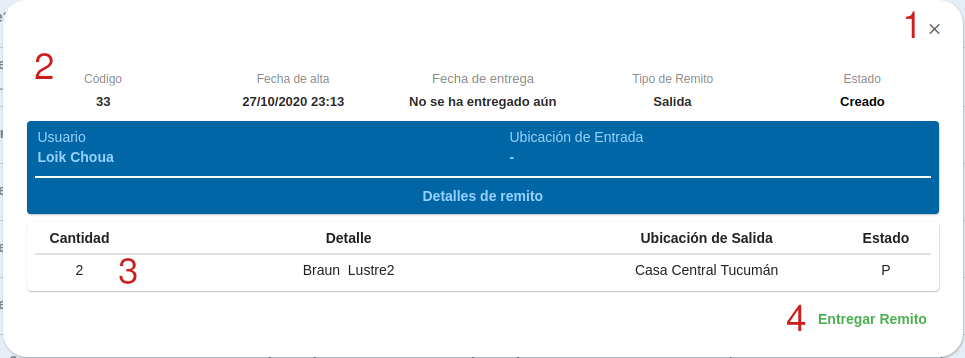
\includegraphics[width=\textwidth,height=\textheight,keepaspectratio]{Escenarios/AD-19-00}
\caption{Escenario - AD-19-00}
\label{fig:AD-19-00}
\end{figure}
Este es el escenario que muestra información más detallada de una remito a los usuarios.
Con el botón \textbf{AD-19-01} se podrá cerrar la ventana y volver al escenario \textbf{AD-16-00}. La sección \textbf{AD-19-02} muestra información relacionado al remito, como ser el código de identificación, fecha de creación, la fecha de entrega o un guion en caso de no haber sido entregado, el tipo de remito, el estado en el cual se encuentra, el usuario que creo el remito y la ubicación en caso de ser un remito del tipo 'Entrada'.
En la sección \textbf{AD-19-03} se muestra infomación de las líneas de remito, como la cantidad, el detalle, la ubicación de salida, en caso de ser un remito de salida, y el estado de la linea de venta. Un click en el boton \textbf{AD-19-04} permite marcar un remito como entregado en caso de estar en el estado 'Creado' y navega al escenario \textbf{AD-16-00}. 
\\